\chapter{metodologia}




\section{Analisis}



\subsection{Requisitos funcionales}
1.-El sistema permitir\'a visualizar a todos los usuarios los precios y promociones de los platillos del restaurante in la necesidad de loguearse en la aplicaci\'on.

2.-El sistema permitir\'a solo a los usuarios registrados la autorizaci\'on de poder reservar una mesa hasta un d\'ia antes.

3.-el sistema permitir\'a solo a los usuarios registrados la autorizaci\'on de poder hacer pedidos a domicilio.



\subsection{Requisitos no funcionales}
1.-La aplicaci\'on debe ser capaz de proporcionar mensajes de error a los usuarios

2.- El sistema no revelara a sus operadores otros datos personales de los clientes..

3.-La aplicaci\'on debe tener una interfaz basada en material design






\section{diseño}


\subsection{Diagrama casos de uso}

\begin{figure}[H]
\caption{diagrama casos de uso}
\centering
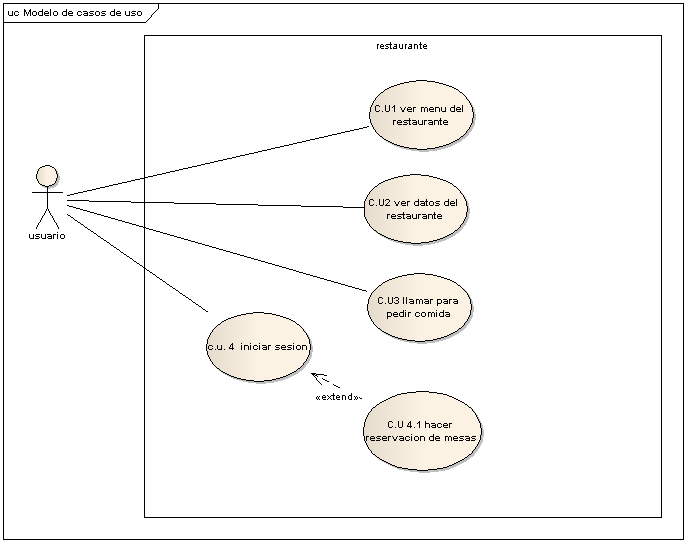
\includegraphics[width=10cm]{imagenes/casosdeuso}

\end{figure}
\subsection{mockup}



\begin{figure}[H]
\caption{mockoup}
\centering
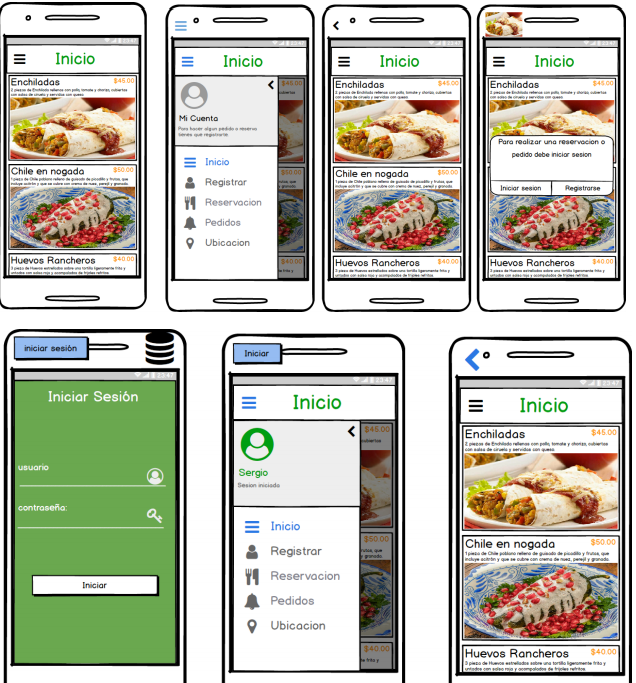
\includegraphics[width=10cm]{imagenes/mockup1}

\end{figure}

\begin{figure}[H]
\caption{mockoup}
\centering
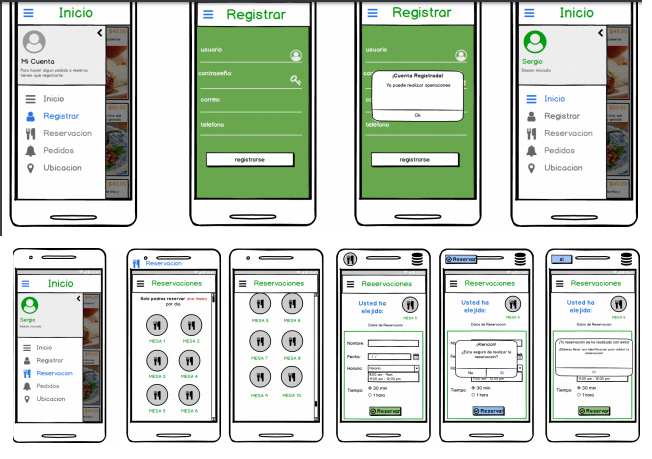
\includegraphics[width=10cm]{imagenes/mockup2}

\end{figure}

\begin{figure}[H]
\caption{mockoup}
\centering
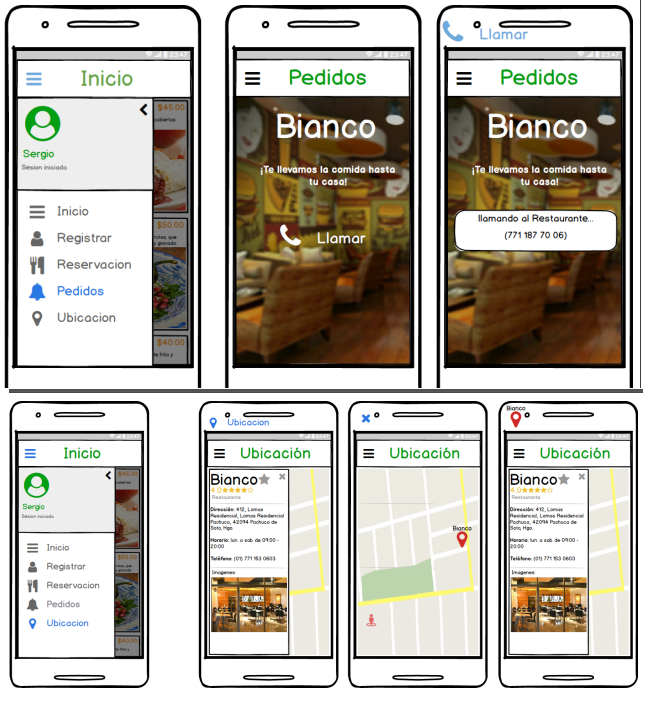
\includegraphics[width=10cm]{imagenes/mockup3}

\end{figure}





\subsection{diagrama de actividades}



\begin{figure}[H]
\caption{diagrama de actividades}
\centering
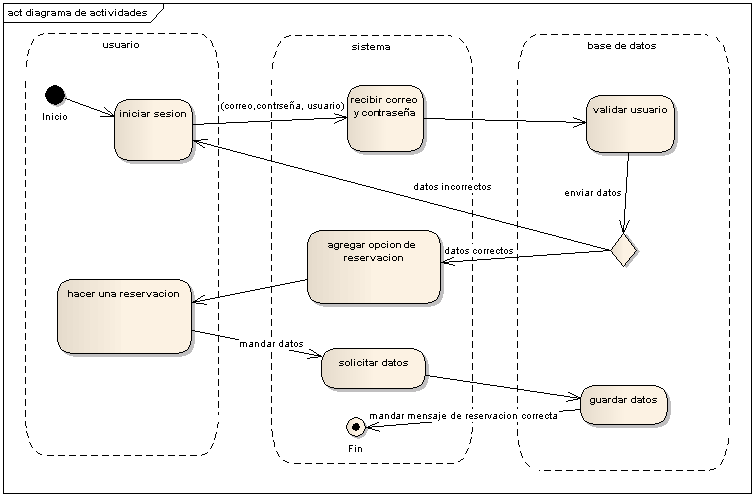
\includegraphics[width=10cm]{imagenes/actividades}

\end{figure}


\subsection{diagrama de secuencias}

\begin{figure}[H]
\caption{diagrama de secuencias}
\centering
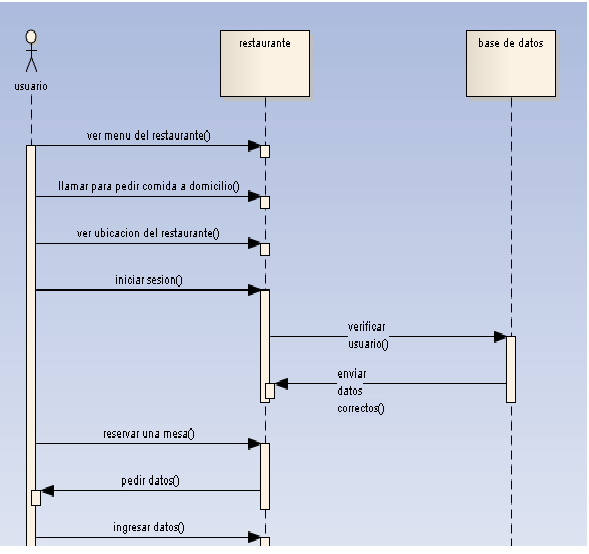
\includegraphics[scale=0.80]{imagenes/secuencias}

\end{figure}




\section{programación}


Para realizar la programación de esta aplicación usaremos Android Studio.

\begin{figure}[H]
\caption{estructura del proyecto}
\centering
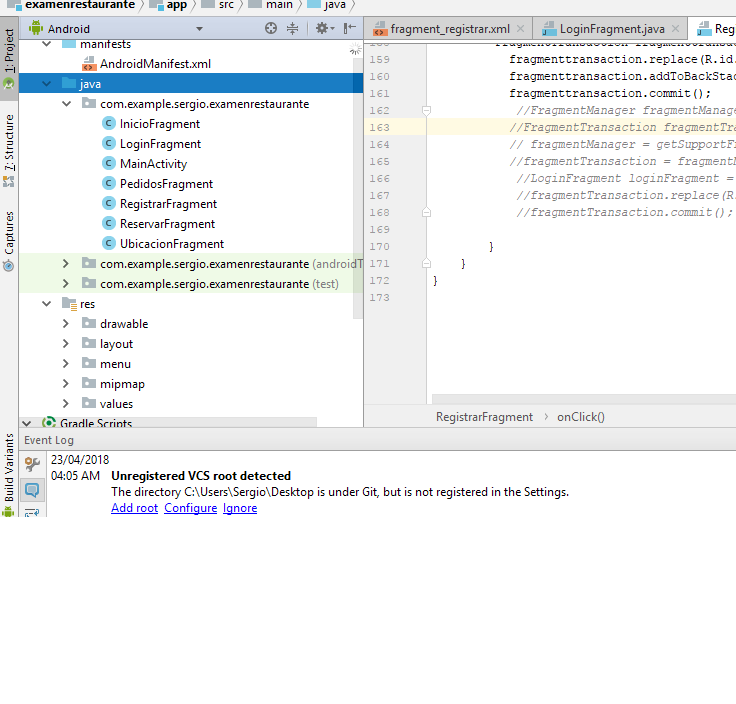
\includegraphics[scale=0.80]{imagenes/programacion}

\end{figure}

\begin{figure}[H]
\caption{layouts}
\centering
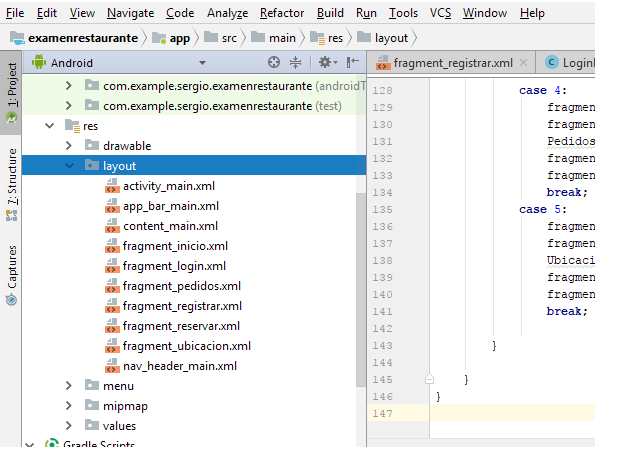
\includegraphics[scale=0.80]{imagenes/programacion2}

\end{figure}


